\documentclass[a4paper,NoNotes,GeneralMath,12pt]{stdmdoc}

\newcommand\cost{\text{cost}}
\makeatletter \newcommand{\vo}{\vec{o}\@ifnextchar{^}{\,}{}} \makeatother
\newenvironment{dtable}{
		\newcommand\dnext{\hfill}
	}{ \\ }

\usepackage{bbm}
\usepackage{setspace}
\usepackage{cancel}
\usepackage{float}
\usepackage{graphicx}
\usepackage[pass]{geometry}

\onehalfspace

\begin{document}
	\title{Cose di Cose}
	
	\section*{Coordinate Polari}
	$\begin{array}{cccc} \vec{r} = r\hat{r} & \vec{\omega} = \dot{\theta} \hat{z} & \vec{v} = \dot{r}\hat{r} + r\dot{\theta}\hat{\theta} & \vec{a} = \left(\ddot{r} - r{\dot{\theta}}^2\right)\hat{r} + \left(2\dot{r}\dot{\theta} + r\ddot{\theta}\right)\hat{\theta} \end{array}$

	\section*{Coordinate Sferiche}
	$\begin{array}{cc} \vec{r} = r\hat{r} & \vec{\omega} = \dot\varphi \hat{z} + \dot\theta \hat\varphi = \dot{\varphi} \left(\cos\theta \hat{r} - \sin\theta \hat{\theta}\right) + \dot{\theta} \hat{\varphi} \end{array}$

	\section*{Campo Centrale}
	$\begin{array}{ccc} \vec{F} = f\left(\mid \vec{r} \mid\right) \hat{r} & \vec{L_0} = \vec{\cost} & V = - \int_{z_0}^{z} f\left(\mid \vec{r} \mid\right) \de{\vec{r}} \end{array}$ \\ 
	$\nabla V = \left(\dpar{V}{x}, \dpar{V}{y}, \dpar{V}{z}\right) = \dpar{V}{r} \left(\dpar{r}{x}, \dpar{r}{y}, \dpar{r}{z}\right) = - f\left(\mid \vec{r} \mid\right) \left(\frac{x}{r}, \frac{y}{r}, \frac{z}{r}\right) = - f\left(\mid \vec{r} \mid \right) \hat{r}$

	\section*{Potenziale Efficace}
	$\begin{array}{cc} \text{Sapendo che } \vec{L} = mr^2 \dot{\theta} \hat{z} & E = \frac{1}{2} m\left({\dot{r}}^2 + r^2 {\dot{\theta}}^2\right) + V\left(r\right) = \frac{1}{2} m {\dot{r}}^2 + \left(\frac{L_z^2}{2mr^2} + V\left(r\right)\right) \end{array}$

	\section*{Viriale}
	$\de{}{t} \left(\vec{r} \cdot \vec{p}\right) = \dot{\vec{r}} \cdot \vec{p} + \vec{r} \cdot \vec{F} = \vec{v} \cdot m\vec{v} - \vec{r} \cdot \nabla V = 2T - \alpha V$ \\ $V\left(\lambda x_1, \ldots, \lambda x_n\right) = \lambda^\alpha V\left(x_1, \ldots, x_n\right)$ \\ $\frac{1}{\tau}\left(\vec{r}\cdot\vec{p}\right) = 2 \langle T \rangle - \alpha \langle V \rangle$ e passando al limite in $\tau \rar 0$ (siccome $\left(\vec{r}\cdot\vec{p}\right)$ è limitato poiché per ipotesi il moto (ovvero $\vec{r}$) è limitato e $\vec{p}$ anche (essendo la massa limitata e la velocità anch'essa periodica e quindi limitata)) $\implies 2 \langle T \rangle = \alpha \langle V \rangle$

	\section*{Conservazione dell'Energia}
	$\begin{array}{cc} E = \frac{1}{2} m {\dot{x}}^2 + V\left(x\right) & \de{E}{t} = m\dot{x}\ddot{x} + \dpar{V}{x} \de{x}{t} = \left(m \ddot{x} - F\right) \dot{x} = 0 \end{array}$

	\section*{Identità del Cazzo}
	$A \cdot \left(B \times C\right) = B \cdot \left(C \times A\right) = C \cdot \left(A \times B\right)$ \\ $A \times \left(B \times C\right) = B\left(A \cdot C\right) - C \left(A \cdot B\right)$ \\ $\varepsilon_{\alpha\beta\gamma} \varepsilon_{\alpha\rho\sigma} = \delta_{\beta\rho}\delta_{\gamma\sigma} - \delta_{\beta\sigma}\delta_{\gamma\rho}$

	\section*{Lagrangiana}
	$\begin{array}{cc} \cL = \sum_i \frac{1}{2} m_i {\dot{q}}_i^2 - V\left(q_i\right) & \de{}{t}\left(\dpar{\cL}{\dot{q}_i}\right) = \dpar{\cL}{q_i} \implies \de{}{t}\left(m_i {\dot{q}_i}\right) = - \dpar{V}{q_i} \implies m_i {\ddot{q}_i} = F_i \end{array}$

	\subsection*{Invarianza nel tempo}
	$\begin{array}{ccc} \cL\left(q, \dot{q}_i\right) & \dpar{\cL}{t} = 0 & E = \dpar{\cL}{\dot{q}} \dot{q} - \cL \end{array}$ \\
	$\de{E}{t} = \de{}{t}\left(\dpar{\cL}{\dot{q}}\right) \dot{q} + \dpar{\cL}{\dot{q}} \ddot{q} - \de{\cL}{t} = \de{}{t}\left(\dpar{\cL}{\dot{q}}\right) \dot{q} + \cancel{\dpar{\cL}{\dot{q}} \ddot{q}} - \dpar{\cL}{q} \dot{q} - \cancel{\dpar{\cL}{\dot{q}} \ddot{q}} = \dot{q} \left(\de{}{t} \left(\dpar{\cL}{\dot{q}}\right) - \dpar{\cL}{q}\right) = 0$

	\subsection*{Invarianza per traslazioni}
	$r_i \mapsto r_i + \varepsilon \delta_i$ \\ $\cL \left(r_i + \varepsilon \delta_i, \dot{r}_i, t\right) - \cL \left(r_i, \dot{r}_i, t\right) = \dpar{\cL}{r_i} \varepsilon \delta_i = 0 \implies 0 = \dpar{\cL}{r_i} = \de{}{t} \left(\dpar{\cL}{\dot{r}_i}\right) = \de{}{t} \left(m_i \dot{r}_i \right)$

	\subsection*{Invarianza per Rotazioni}
	$\begin{array}{cc} \vec{r}_i \mapsto \left(\mathbbmtt{1} + \delta \vec{\varphi}\times \right) \vec{r}_i & \dot{\vec{r}}_i \mapsto \left(\mathbbmtt{1} + \delta \vec{\varphi} \times\right) {\dot{\vec{r}}_i} \end{array}$ \\
	$\cL\left( \left(\mathbbmtt{1} + \delta \vec{\varphi} \times\right) \vec{r}_i, \left(\mathbbmtt{1} + \delta \vec{\varphi} \times\right) \dot{\vec{r}}_i, t\right) - \cL\left( \vec{r}_i, \dot{\vec{r}}_i, t\right) = \dpar{\cL}{\vec{r}_i} \cdot \delta \vec{\varphi}\times \vec{r}_i + \dpar{\cL}{\dot{\vec{r}}_i} \cdot \delta \vec{\varphi} \times \dot{\vec{r}}_i = \delta \vec{\varphi} \cdot \left( \vec{r}_i \times \dpar{\cL}{\vec{r}_i} + \dot{\vec{r}}_i \times \dpar{\cL}{\dot{\vec{r}}_i} \right) = 0$ \\
	$\vec{r}_i \times \dpar{\cL}{\vec{r}_i} + \dot{\vec{r}}_i \times \dpar{\cL}{\dot{\vec{r}}_i} = 0$ \\ $\vec{r}_i \times \de{}{t} \left( \dpar{\cL}{\dot{\vec{r}}_i} \right) + \dot{\vec{r}}_i \times \dpar{\cL}{\dot{\vec{r}}_i} = \de{}{t} \left( \vec{r}_i \times \dpar{\cL}{\dot{\vec{r}}_i} \right) = \de{}{t} \left( \vec{r}_i \times m_i \dot{\vec{r}}_i \right) = 0$

	\section*{Cambio di Sistema di Riferimento}
	$\begin{array}{ccc} \vec{r}_{\text{lab}} = \vec{R} + \vec{r}_{\text{rel}} & \vec{v}_{\text{lab}} = \vec{V} + \vec{v}_{\text{rel}} + \vec{\omega} \times \vec{r}_{\text{rel}} & \vec{a}_{\text{lab}} = \vec{A} + \vec{a}_{\text{rel}} + 2 \vec{\omega} \times \vec{v}_{\text{rel}} + \dot{\vec{\omega}} \times \vec{r}_{\text{rel}} + \vec{\omega} \times \left( \vec{\omega} \times \vec{r}_{\text{rel}} \right) \end{array}$

	\section*{Formule che valgono sempre (e siamo sicuri perché abbiamo fatto i conti al contrario dei fisici che le tirano fuori dal cappello ma non sanno come dimostrarle)}
	Il sistema di riferimento è $\Sigma = O\hat{x}\hat{y}\hat{z}$. Il punto $P$ è quello rispetto a cui si calcolano $\vec{L}_P$ e $\vec{\tau}_P$. Le particelle $\alpha$ hanno raggio vettore rispetto ad $O$ $\vec{r}_\alpha$ e rispetto a $P$ $\vec{\rho}_\alpha$, quindi $\vec{r}_\alpha = \vec{OP} + \vec{\rho}_\alpha$ \\
	$\vec{L}_P := \sum_\alpha \vec{\rho}_\alpha \times m_\alpha \dot{\vec{r}}_\alpha , \quad \vec{\tau}_P := \sum_\alpha \vec{\rho}_\alpha \times m_\alpha \ddot{\vec{r}}_\alpha$ \\
	$\vec{L}_P = \sum_\alpha \vec{\rho}_\alpha \times m_\alpha \dot{\vec{r}}_\alpha = \sum_\alpha \left( \vec{r}_\alpha - \vec{OP} \right) \times m_\alpha \dot{\vec{r}}_\alpha = \sum_\alpha \vec{r}_\alpha \times m_\alpha \dot{\vec{r}}_\alpha - \sum_\alpha \vec{OP} \times m_\alpha \dot{\vec{r}}_\alpha = \vec{L}_O - \vec{OP} \times \vec{P}$ \\
	$\left. \de{\vec{L}_P}{t}\right|_\Sigma = \sum_\alpha \dot{\vec{\rho}}_\alpha \times m_\alpha \dot{\vec{r}}_\alpha +\sum_\alpha {\vec{\rho}}_\alpha \times m_\alpha \ddot{\vec{r}}_\alpha = \vec{\tau}_P + \cancel{\sum_\alpha \dot{\vec{r}}_\alpha \times m_\alpha \dot{\vec{r}}_\alpha } - \sum_\alpha \dot{\vec{OP}} \times m_\alpha \dot{\vec{r}}_\alpha = \vec{\tau}_P - \dot{\vec{OP}} \times \vec{P}$

	\section*{Problema dei due Corpi}
	Assunzioni: 
	\begin{enumerate}
		\item Corpi puntiformi
		\item Il potenziale dipende solo dalla distanza relativa
	\end{enumerate}
	$E = \frac{1}{2} m_1 {\dot{\vec{r}}_1}^2 + \frac{1}{2} m_2 {\dot{\vec{r}}_2}^2 + V \left( \mid \vec{r}_2 - \vec{r}_1 \mid \right)$ \\ $\left\{ \begin{array}{cc} \vec{r} = \vec{r}_2 - \vec{r}_1 & \vec{R} = \frac{m_1 \vec{r}_1 + m_2 \vec{r}_2}{m_1 + m_2} \\ \mu = \frac{m_1 m_2}{m_1 + m_2} & M = m_1 + m_2 \end{array} \right\}$ \\ $\left( \begin{array}{c} \vec{r}_1 \\ \vec{r}_2 \end{array} \right) = \left( \begin{array}{cc} \frac{m_2}{m_1 + m_2} & 1 \\ \frac{m_1}{m_1 + m_2} & 1 \end{array} \right) \left( \begin{array}{c} \vec{r} \\ \vec{R} \end{array} \right)$ \\
	$E = \frac{1}{2} M {\dot{\vec{R}}}^2 + \frac{1}{2} \mu {\dot{\vec{r}}}^2 + V \left( \mid \vec{r} \mid \right)$ \\ $L = \vec{R} \times M \dot{\vec{R}} + \vec{r} \times \mu \dot{\vec{r}}$

	\section*{Urti}

	Fatti incredibili:
	\begin{enumerate}
		\item La $\vec{p}$ si conserva sempre (non ci sono forze esterne)
		\item Per definizione, se l'urto è elastico, l'energia si conserva
	\end{enumerate}

	\begin{itemize}
		\item $m_1, \quad \vec{v}_1, \quad m_2, \quad \vec{v}_2$ \\ masse e velocità relative al sistema del laboratorio.
		\item $\vec{v} := \vec{v}_1 - \vec{v}_2, \qquad \vec{R} := \frac{m_1\vec{r}_1 + m_2\vec{r}_2}{m_1 + m_2}, \qquad \vec{V} = \dot{\vec{R}}, \qquad \mu := \frac{m_1m_2}{m_1+m_2}$
		\item $m_1, \quad \vec{v}_{10} = \vec{v}_1 - \vec{V} = \frac{m_2}{m_1 + m_2} \vec{v}, \quad m_2, \quad \vec{v}_{20} = \vec{v}_2 - \vec{V} = -\frac{m_1}{m_1 + m_2} \vec{v}$ \\ masse e velocità relative al sistema del centro di massa.
		\item $\vec{p}_1 = \mu \vec{v} + m_1 \vec{V} \qquad \vec{p}_2 = -\mu \vec{v} + m_2 \vec{V}$
		\item $\vec{p}_{10} = \vec{p}_1 - m_1\vec{V} = m_1 \vec{v}_{10} = \frac{m_2m_1}{m_1 + m_2} \vec{v} = \mu \vec{v}, \qquad \vec{p}_{20} = \vec{p}_2 - m_2\vec{V} = m_2 \vec{v}_{20} = -\frac{m_1m_2}{m_1 + m_2} \vec{v} = - \mu \vec{v}$
		\item $\vec{v}'_{10} = \frac{m_2}{m_1 + m_2} v \hat{n_0}, \qquad \vec{v}'_{20} = - \frac{m_1}{m_1 + m_2} v \hat{n_0}$
		\item $\vec{v}'_1 = \vec{v}'_{10} + \vec{V} = \frac{m_2}{m_1 + m_2} v \hat{n_0} + \frac{m_1\vec{v}_1 + m_2 \vec{v}_2}{m_1 + m_2}, \qquad \vec{v}'_2 = \vec{v}'_{20} + \vec{V} = - \frac{m_1}{m_1 + m_2} v \hat{n_0} + \frac{m_1\vec{v}_1 + m_2\vec{v}_2}{m_1 + m_2}$
		\item $\vec{p}'_1 = m_1\vec{v}'_1 = \mu v \hat{n_0} + \frac{m_1}{m_1 + m_2} \vec{P} = \mu v \hat{n_0} + m_1 \vec{V}, \qquad \vec{p}'_2 = m_2 \vec{v}'_2 = - \mu v \hat{n_0} + \frac{m_2}{m_1+m_2} \vec{P} = - \mu v \hat{n_0} + m_2 \vec{V}$
	\end{itemize}

	\section*{Puttanate sugli angoli}

	\begin{minipage}{0.6\textwidth}
	\subsection*{CM Frame}
	Angolo qualsiasi. Le palline possono andare dove vogliono.

	\subsection*{LAB Frame}
	L'angolo è limitato. $\sin \theta_{\text{max}} = \frac{\mu v}{m_1 V} = \frac{m_1 v_{10}}{m_1 V} = \frac{v_{10}}{V}$
	\end{minipage}
	\hfill
	\begin{minipage}{0.35\textwidth}
	\begin{figure}[H]
		\centering
		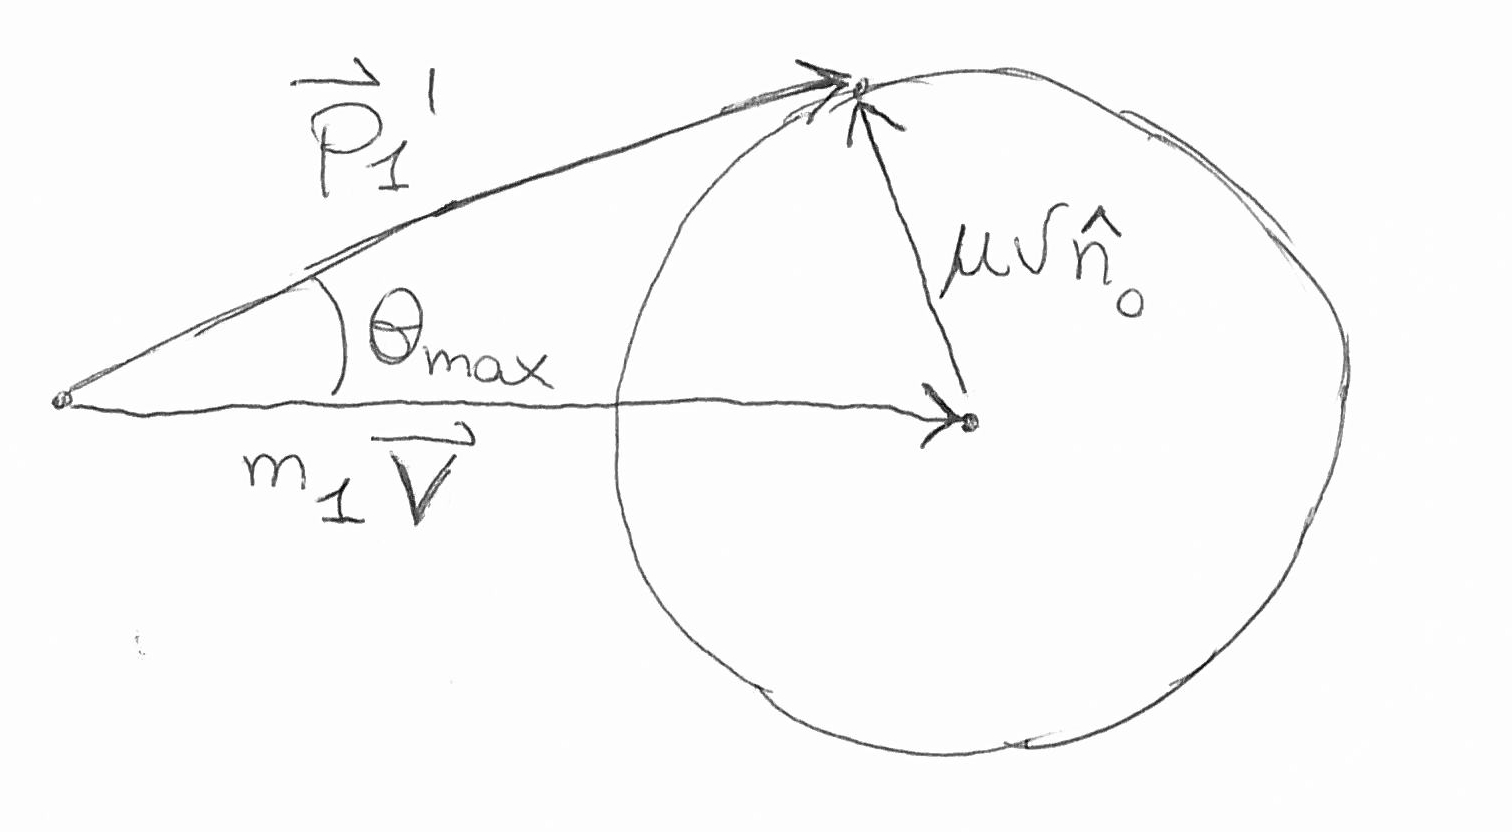
\includegraphics[width=\columnwidth]{AngoloMagico}
	\end{figure}
	\end{minipage}

	\section*{Problemi con massa variabile}
	Cosa utile: $\vec{F} = \dot{\vec{p}}$ \\
	$\vec{v}_\text{agg}$ è la velocità assoluta della particella che si sta aggiungendo \\
	$\left( m + \de m \right) \left( \vec{v} + \de \vec{v} \right) - m \vec{v} - \de m \vec{v}_\text{agg} = \vec{F}^{(E)} \de t$ \\
	$\de{m} \left( \vec{v} - \vec{v}_\text{agg} \right) + m \de{\vec{v}} = \vec{F}^{(E)} \de{t}$ \\
	$\left( \vec{v} - \vec{v}_\text{agg} \right) \de{m}{t} + m \vec{a} = \vec{F}^{(E)}$

	\section*{Tensore d'Inerzia}
	$T_{ij} = R_{ik} R_{jl} T_{kl}$ \\ $I_{ij} = \sum_\alpha m^{\alpha} \left( r_k^\alpha r_k^\alpha \delta_{ij} - r_i^\alpha r_j^\alpha \right)$

	\section*{Oscillazioni a più gradi di libertà}
	Equazione: $M_{ij} \ddot{x}_j = -K_{ij} x_j$ \\
	Claim: $x_j = A_j e^{i\omega t}$ \\
	$M_{ij} A_j i^2 \omega^2 e^{i\omega t} = - K_{ij} A_{j} e^{i\omega t}$ \\
	$\left(M_{ij} \omega^2 - K_{ij} \right) A_j = 0$ \\
	Vogliamo $A \neq 0$ quindi $\Det (M\omega^2 - K) = 0$. Risolviamo ora per gli $\omega$ poi troviamo gli $A$ come $\Ker (M\omega^2 - K )$. \\
	Troviamo $n$ vettori $A$. Adesso ho che una generica soluzione si scrive come $\left(\tilde{X}\right) = \sum_\alpha c_\alpha e^{i\omega t} \left( A^\alpha \right) = \left( A \right) \left( \begin{array}{c} c_1 e^{i\omega_1 t} \\ \vdots \\ c_n e^{i\omega_n t} \end{array} \right)$ \\
	Ora, invertendo la matrice $A$ trovo $\left( \begin{array}{c} c_1 e^{i\omega_1 t} \\ \vdots \\ c_n e^{i\omega_n t} \end{array} \right) = \left( A^{-1} \right) \left( \tilde{X} \right)$ \\
	Quindi definisco le mie nuove coordinate (che oscillano con frequenze "pure") come $\left( Q \right) = \left( A^{-1} \right) \left( X \right)$. L'energia è diagonale: $E = \sum_\alpha \frac{1}{2} m_\alpha ({\dot{q}_\alpha^2} + \omega_\alpha^2 q_\alpha^2 )$

	\section*{Termodinamica}
	\subsection*{Leggi Universali}
	$\Delta U = Q - L^{\vec{}} \qquad U = n C_V T = \frac{1}{\gamma -1} nRT$ \\
	$\Delta S = nC_V \log \left( \frac{T_2}{T_1} \right) + n R \log \left( \frac{V_2}{V_1} \right) \qquad \Delta S = n C_P \log \left( \frac{T_2}{T_1} \right) - n R \log \left( \frac{p_2}{p_1} \right)$

	\subsection*{Isobara ($p$ costante)}
	$\Delta U = n C_V \Delta T \qquad Q = n C_P \Delta T \qquad L^{\vec{}} = nR \Delta T = p \Delta V \qquad \Delta S = n C_P \log \left( \frac{T_2}{T_1} \right)$
	
	\subsection*{Isoterma ($T$ costante)}
	$\Delta U = 0 \implies Q = L^{\vec{}} \qquad Q = nRT \log \left( \frac{V_2}{V_1} \right) \qquad L^{\vec{}} = nRT \log \left( \frac{V_2}{V_1} \right) \qquad \Delta S = nR \log \left( \frac{V_2}{V_1} \right) $

	\subsection*{Isocora ($V$ costante)}
	$\Delta U = n C_V \Delta T \qquad Q = n C_V \Delta T \qquad L^{\vec{}} = 0 \qquad \Delta S = n C_V \log \left( \frac{T_2}{T_1} \right)$

	\subsection*{Adiabatica reversibile (senza scambio di calore)}
	$\Delta U = n C_V \Delta T \qquad Q = 0 \qquad L^{\vec{}} = n C_V \Delta T = \frac{\Delta (pV)}{1 - \gamma}$ \\ $pV^\gamma = \text{cost} \qquad TV^{\gamma -1} = \text{cost} \qquad pT^{\frac{\gamma}{1-\gamma}} = \text{cost}$

	\section*{Relazioni sui $\de$ qualcosa}
	$\de{U} + \de{L^{\vec{}}} = \de{Q}, \quad pV = nRT \implies p\de{V} + V\de{p} = nR\de{T}, \quad \de{L^{\vec{}}} = p\de{V}, \quad \de{U} = nC_V \de{T}$ \\
	$\de{U} \frac{R}{C_V} = nR\de{T} = \de{L^{\vec{}}} + V\de{p} = \de{Q} - \de{U} + V\de{p} \implies \de{Q} = nC_P \de{T} - V\de{p}$

\end{document}
